\begin{pr}
Let's modify the proof in class.\\
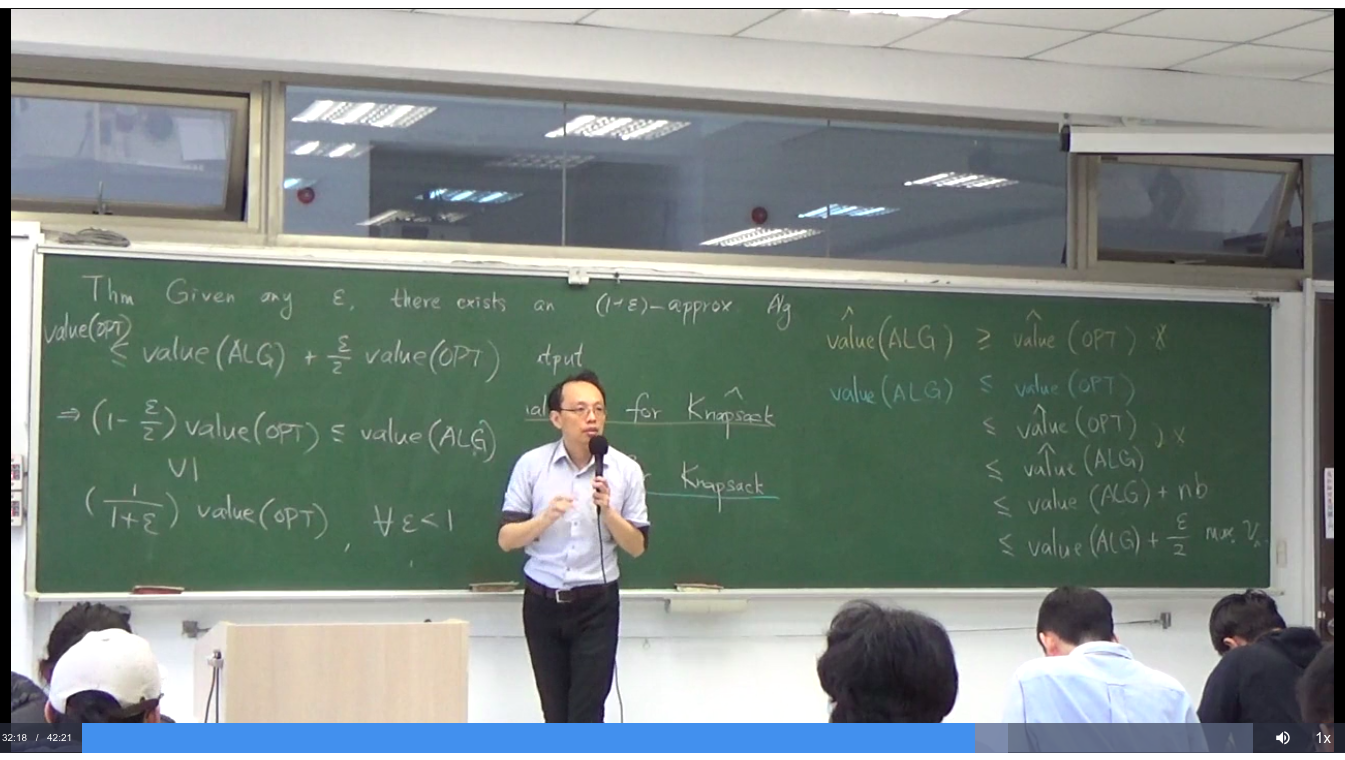
\includegraphics[width=15cm]{p3.png}\\
In class, we learn that we can use greedy algorithm to get a $2$-approximation.\\
That is, we know a $k$ such that $k\leq val(OPT)\leq2k$.\\
Take $b=\frac{\epsilon k}{2n}$.\\
$\then value(ALG)\leq value(OPT)\leq\hat{value}(OPT)\leq\hat{value}(ALG)\leq value(ALG)+nb\leq value(ALG)+\frac{\epsilon k}2\leq value(ALG)+\frac\epsilon2value(OPT)$ still holds.\\
$\then$ this is still an $(1+\epsilon)$-approximation.\\
Time complexity:\\
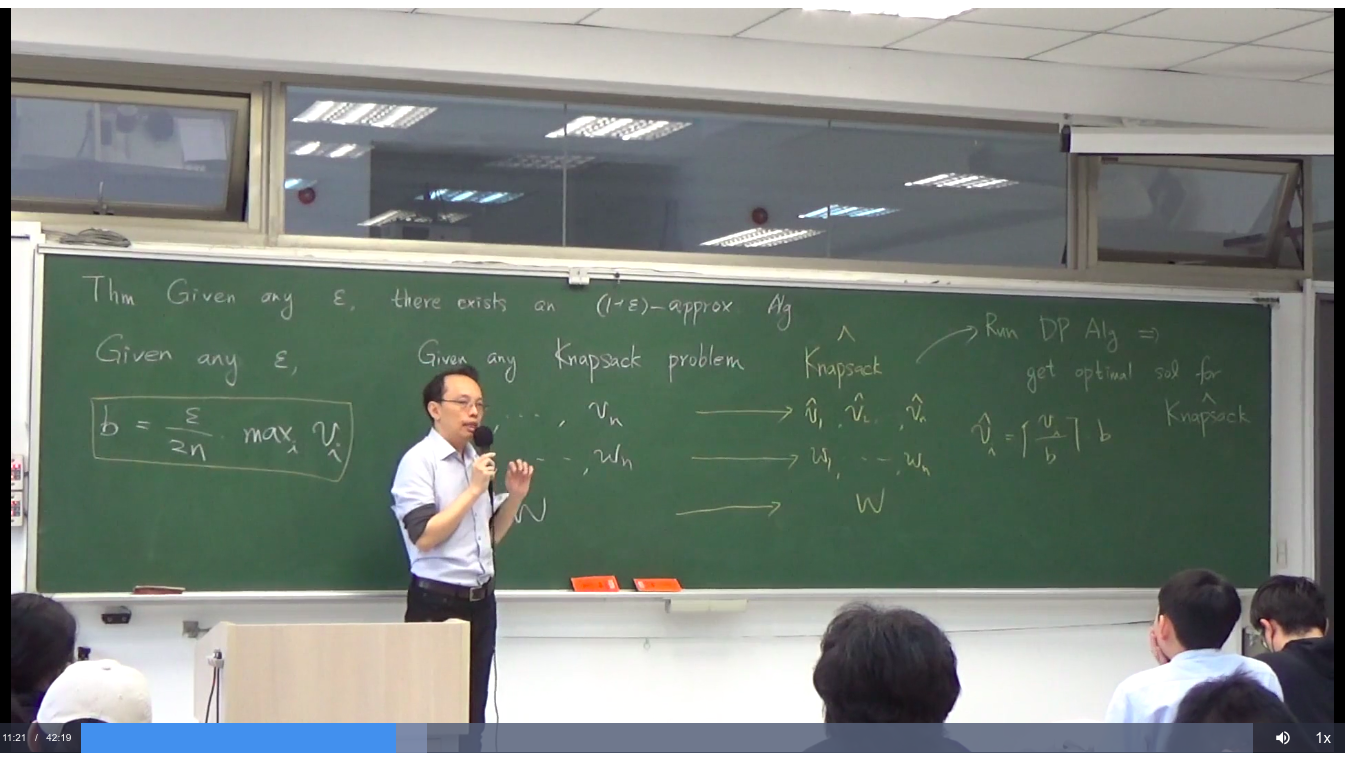
\includegraphics[width=15cm]{p3t0.png}\\
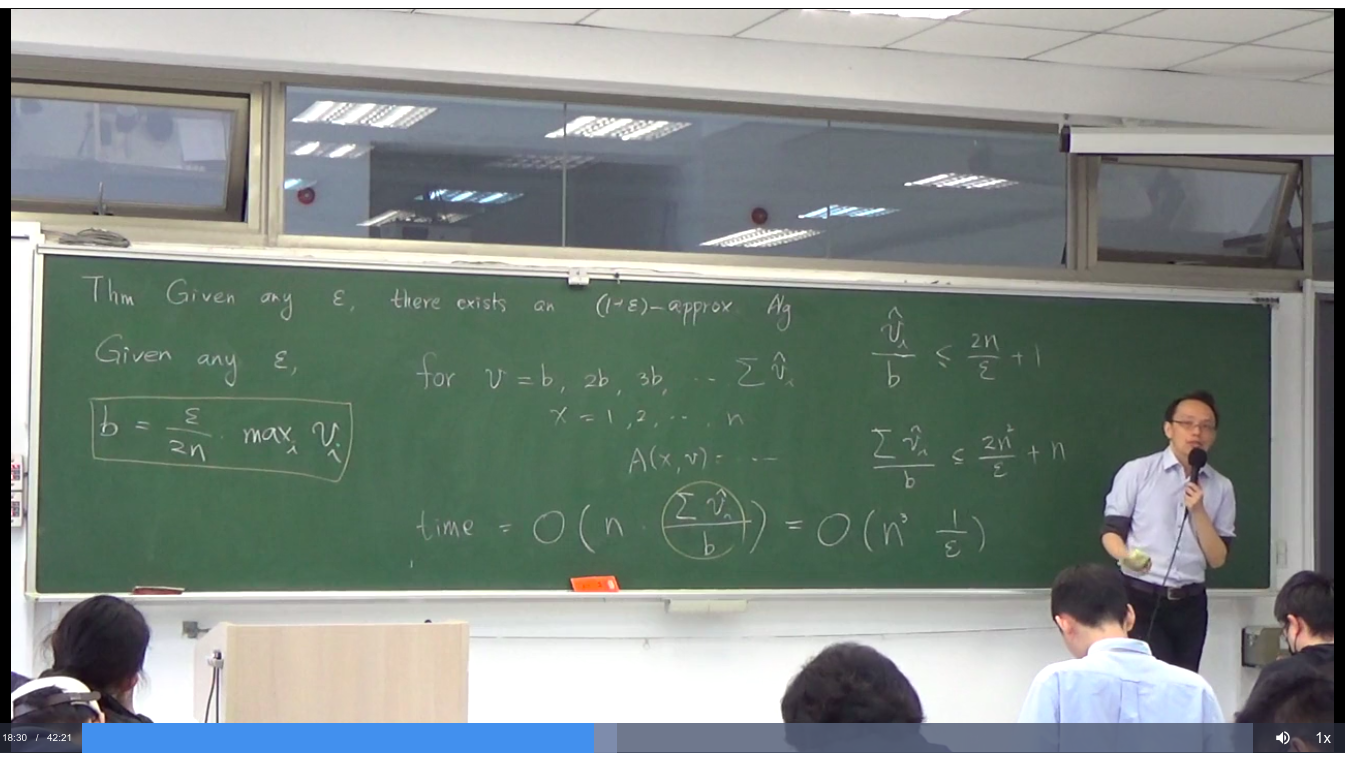
\includegraphics[width=15cm]{p3t.png}\\
The upperbound of $v$ in $A(x, v)$ in the DP algorithm changed from $\frac{\suml\hat v_n}b$ to $\lceil\frac{3k}b\rceil$, since we know that $\hat{value}(ALG)\leq value(ALG)+\frac{\epsilon}2value(OPT)\leq(1+\frac\epsilon2)value(OPT)\leq(1+\frac\epsilon2)2k=2k+\epsilon k\leq3k$.\\
Time complexity $=O(n\frac{3k}b)=O(n\frac{3k\times2n}{\epsilon k})=O(\frac{n^2}\epsilon)$.
\end{pr}
